\documentclass[11pt]{article}
\usepackage[margin=0.86in]{geometry}
\usepackage{amsmath,amssymb,booktabs,graphicx,microtype,tabularx,array}
\usepackage{xcolor}
\usepackage[hidelinks]{hyperref}
\graphicspath{{figures/}}
\setlength{\parindent}{0pt}
\setlength{\parskip}{0.52em}
\newcommand{\E}{\mathbb E}
\newcommand{\Prob}{\mathbb P}
\newcommand{\sm}{\Sigma^{\mathrm m}}
\newcommand{\stot}{\Sigma^{\mathrm{tot}}}

\title{Mentor Round-II Report:\\
Two-tail Flux Statistics and Fluctuation-Theorem Diagnostics\\
for the Boundary-driven Resonant NLS Chain}
\author{Detailed numerical report and reproducibility package}
\date{30 August 2026}

\begin{document}
\maketitle

\begin{abstract}
This report answers the mentor's second-round questions about the two tails of
the finite-time flux distribution and whether the boundary-driven resonant
NLS chain follows a fluctuation theorem.  For each
$n=10,20,30,40$, we generated $1{,}000{,}064$ non-overlapping blocks of
length $20$ after burn-in and aggregated them to
$\tau=20,40,\ldots,200$.  The central distribution is increasingly
Gaussian-like, but the $\tau=20$ far tails are heavier than the Gaussian fixed
by the full-sample variance.  Wherever raw tail counts remain adequate,
$\log P_\tau$ is approximately linear in $\tau$ at fixed threshold, giving
resolved finite-time large-deviation rate proxies.  Direct medium-entropy and
heat-current symmetry slopes do not reach their asymptotic references before
the negative tails become unresolved, so direct sampling alone gives ``not
verified in the accessible window'', not a violation.  Two independent
$n=2$ total-entropy calculations pass finite-time detailed and integral
fluctuation-relation audits.  Finally, controlled cloning calculations at
$n=10,20,30,40$ pass all frozen support and convergence gates and are
numerically consistent with the Gallavotti--Cohen SCGF symmetry at one
resolved complementary tilt pair per length.  The latter is a finite-size,
tested-window numerical statement, not an all-tilt proof or a thermodynamic-
limit theorem.
\end{abstract}

\section{The mentor's questions and the implemented answer}

The requested workflow was:
\begin{enumerate}
\item after burn-in, store a long trajectory and form approximately $10^6$
      samples of the flux measured over segments of length $20$;
\item describe the central $1$--$99\%$ distribution by a histogram;
\item compare both tails with a normal survival function;
\item use a finite-count correction when a tail count is small;
\item plot the positive and negative probabilities and test their dependence
      on the threshold $A$ and averaging time $\tau$;
\item determine whether the fluctuation-theorem symmetry is supported.
\end{enumerate}

All requested data products were generated.  Two technical corrections were
needed to make the test scientifically well defined.  First, adding two
successes and two failures gives the display-only plus-four estimator
\begin{equation}
 \widehat p_{+4}=\frac{k+2}{N+4},
\end{equation}
not $(k+2)/(N+2)$.  The denominator increases by four because four artificial
observations are added in total.  Raw nonzero counts, rather than this
smoothed value, are used in all inferential fits.  Second, the FT diagnostic
is the logarithm of a probability ratio,
\begin{equation}
 \log\frac{p_\tau(A)}{p_\tau(-A)},
 \label{eq:correct-ratio}
\end{equation}
not the ratio $\log p_\tau(A)/\log p_\tau(-A)$.  Equation
\eqref{eq:correct-ratio} is the quantity related to entropy production.

\begin{table}[ht]
\centering
\small
\begin{tabularx}{\textwidth}{>{\raggedright\arraybackslash}p{0.21\textwidth}
>{\raggedright\arraybackslash}p{0.30\textwidth}
>{\raggedright\arraybackslash}X}
\toprule
Mentor request & Implementation & Status and interpretation\\
\midrule
$10^6$ samples at $\tau=20$ & $1{,}000{,}064$ blocks for every $n$, 128 independent streams & complete and audited\\
Central histogram & empirical PDF over the central $1$--$99\%$ region & complete; increasingly Gaussian-like\\
Normal tail fit & empirical survival versus $\overline\Phi((x-\mu)/\sigma)$ and a joint two-tail Gaussian fit & complete; descriptive, not an FT test\\
Small-count correction & $(k+2)/(N+4)$ for visualization only & complete; zero-count tails are not treated as evidence\\
Dependence on $A$ and $\tau$ & threshold grid $0.01,0.02,\ldots$ and $\tau=20,40,\ldots,200$ & complete where raw counts resolve the tail\\
Fluctuation theorem & direct ratio, $n=2$ total entropy, and long-time SCGF cloning & direct test inconclusive; $n=2$ passes; long chains are consistent at tested pairs\\
\bottomrule
\end{tabularx}
\caption{One-to-one map from the mentor's request to the completed analyses.}
\end{table}

\section{Dynamics, heat, entropy, and current}

All accepted samplers use projection-free Cartesian variables
$c_j=x_j+i y_j$.  There is no action floor or positivity projection.  The
bath parameters are
\begin{equation}
 (T_L,T_R,\gamma)=(10,2,0.1),\qquad \Delta t=5\times10^{-4},
\end{equation}
unless a timestep control is explicitly stated.  The direct production uses
burn-in $B=500$.

Bath heat $Q_r$ is accumulated from the energy change across the corresponding
bath-only substep, with heat positive into the chain.  It is not replaced by
the whole-step energy change.  The medium entropy is
\begin{equation}
 \sm_\tau=-\frac{Q_L(\tau)}{T_L}-\frac{Q_R(\tau)}{T_R}.
 \label{eq:medium}
\end{equation}
Every base block stores $Q_L,Q_R,\Delta E,\sm$, the bulk action current,
stream and block identifiers, and the first-law residual
$Q_L+Q_R-\Delta E$.

Three questions must be kept separate:
\begin{itemize}
\item the distribution and large-deviation shape of the action current;
\item the finite-time fluctuation relation for total thermodynamic entropy;
\item the long-time Gallavotti--Cohen symmetry of the entropy-current SCGF.
\end{itemize}
The action current is not assumed to equal entropy production.

\section{Direct two-tail experiment}

\subsection{Sampling and numerical integrity}

For each $n=10,20,30,40$, 128 independent streams produced
$1{,}000{,}064$ non-overlapping $\tau=20$ blocks.  Consecutive base blocks
within each stream were grouped without overlap to form
$\tau=40,60,\ldots,200$.  This preserves the stream identity and avoids
inventing independent samples through a moving window.

The accepted audit found exactly the requested row count, no nonfinite rows,
no midpoint failures, and no ordering errors.  The entropy and first-law
columns recompute from the stored heat and energy columns.  The RMS
first-law-residual rate ranges from $9.71\times10^{-6}$ at $n=10$ to
$3.05\times10^{-6}$ at $n=40$; halving the timestep reduces this residual by
approximately a factor of four.  Equal-temperature and bath-swapped controls
give the expected zero-current and current-reversal behavior.  An independent
analysis audit performed 75,617 checks with zero errors.

\begin{table}[ht]
\centering
\begin{tabular}{rrrrr}
\toprule
$n$ & blocks at $\tau=20$ & $\langle J\rangle$ & heat current & $\langle\sm\rangle/\tau$\\
\midrule
10 & 1,000,064 & 0.39809 & 3.21212 & 1.28485\\
20 & 1,000,064 & 0.11979 & 1.40691 & 0.56275\\
30 & 1,000,064 & 0.05426 & 0.79595 & 0.31839\\
40 & 1,000,064 & 0.03052 & 0.52294 & 0.20918\\
\bottomrule
\end{tabular}
\caption{Production means from the joint Cartesian sampler.}
\label{tab:means}
\end{table}

As an independent transport cross-check, these means obey
\begin{equation}
 \langle J(n)\rangle=28.889\,n^{-1.8485},\qquad R^2=0.9987,
\end{equation}
consistent with the established canonical estimate
$28.75n^{-1.850}$.

\subsection{Central shape and normal-tail benchmark}

For a finite-time current $J_\tau$, the Gaussian survival benchmark is
\begin{equation}
 \Prob(J_\tau\ge A)\approx
 \overline\Phi\!\left(\frac{A-\mu_\tau}{\sigma_\tau}\right).
\end{equation}
The central distribution narrows and looks increasingly Gaussian as $\tau$
grows.  This is compatible with ordinary averaging near the mean.  It does
not imply that the large-deviation tails are Gaussian.

At $\tau=20$, fitting one Gaussian jointly to both empirical far tails requires
a width larger than the full-sample standard deviation by factors
$1.134,1.199,1.257,$ and $1.283$ for $n=10,20,30,40$.  Thus the far tails are
systematically heavier than the Gaussian fixed by the central variance.

\begin{figure}[ht]
\centering
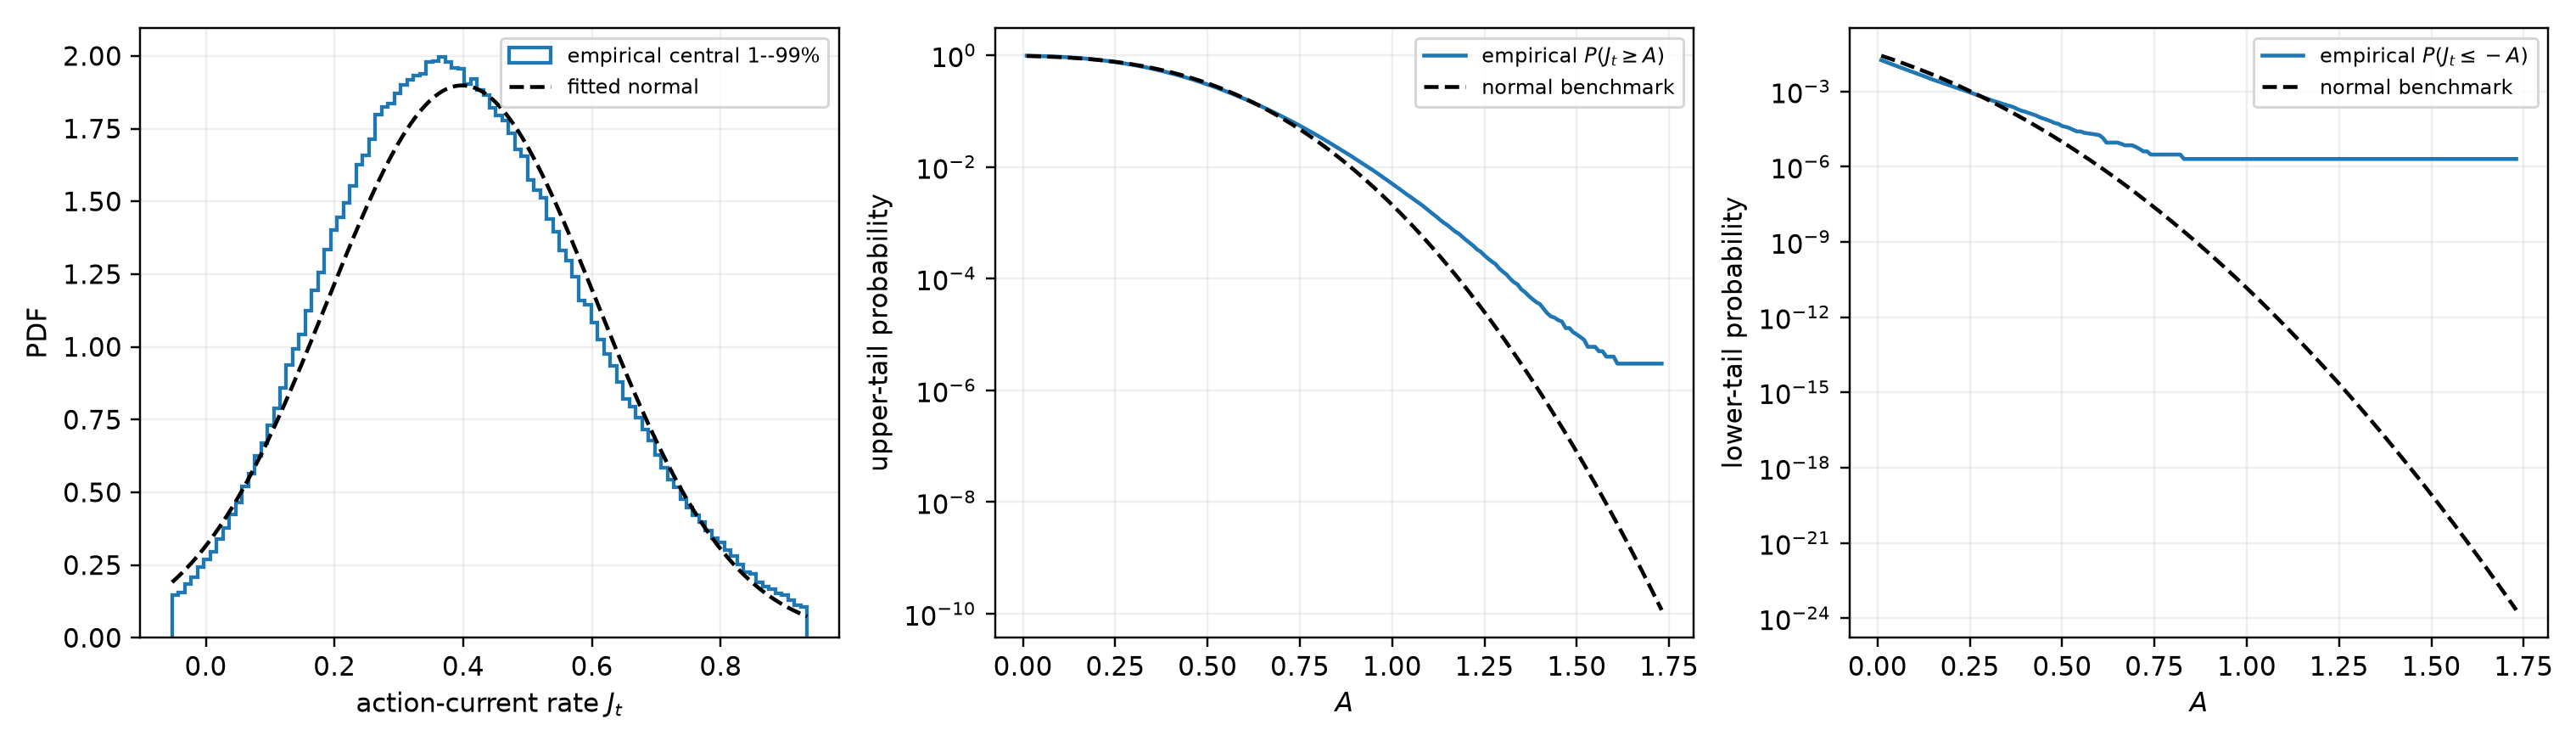
\includegraphics[width=0.48\textwidth]{action_tail_normal_fit_n10_t20.png}\hfill
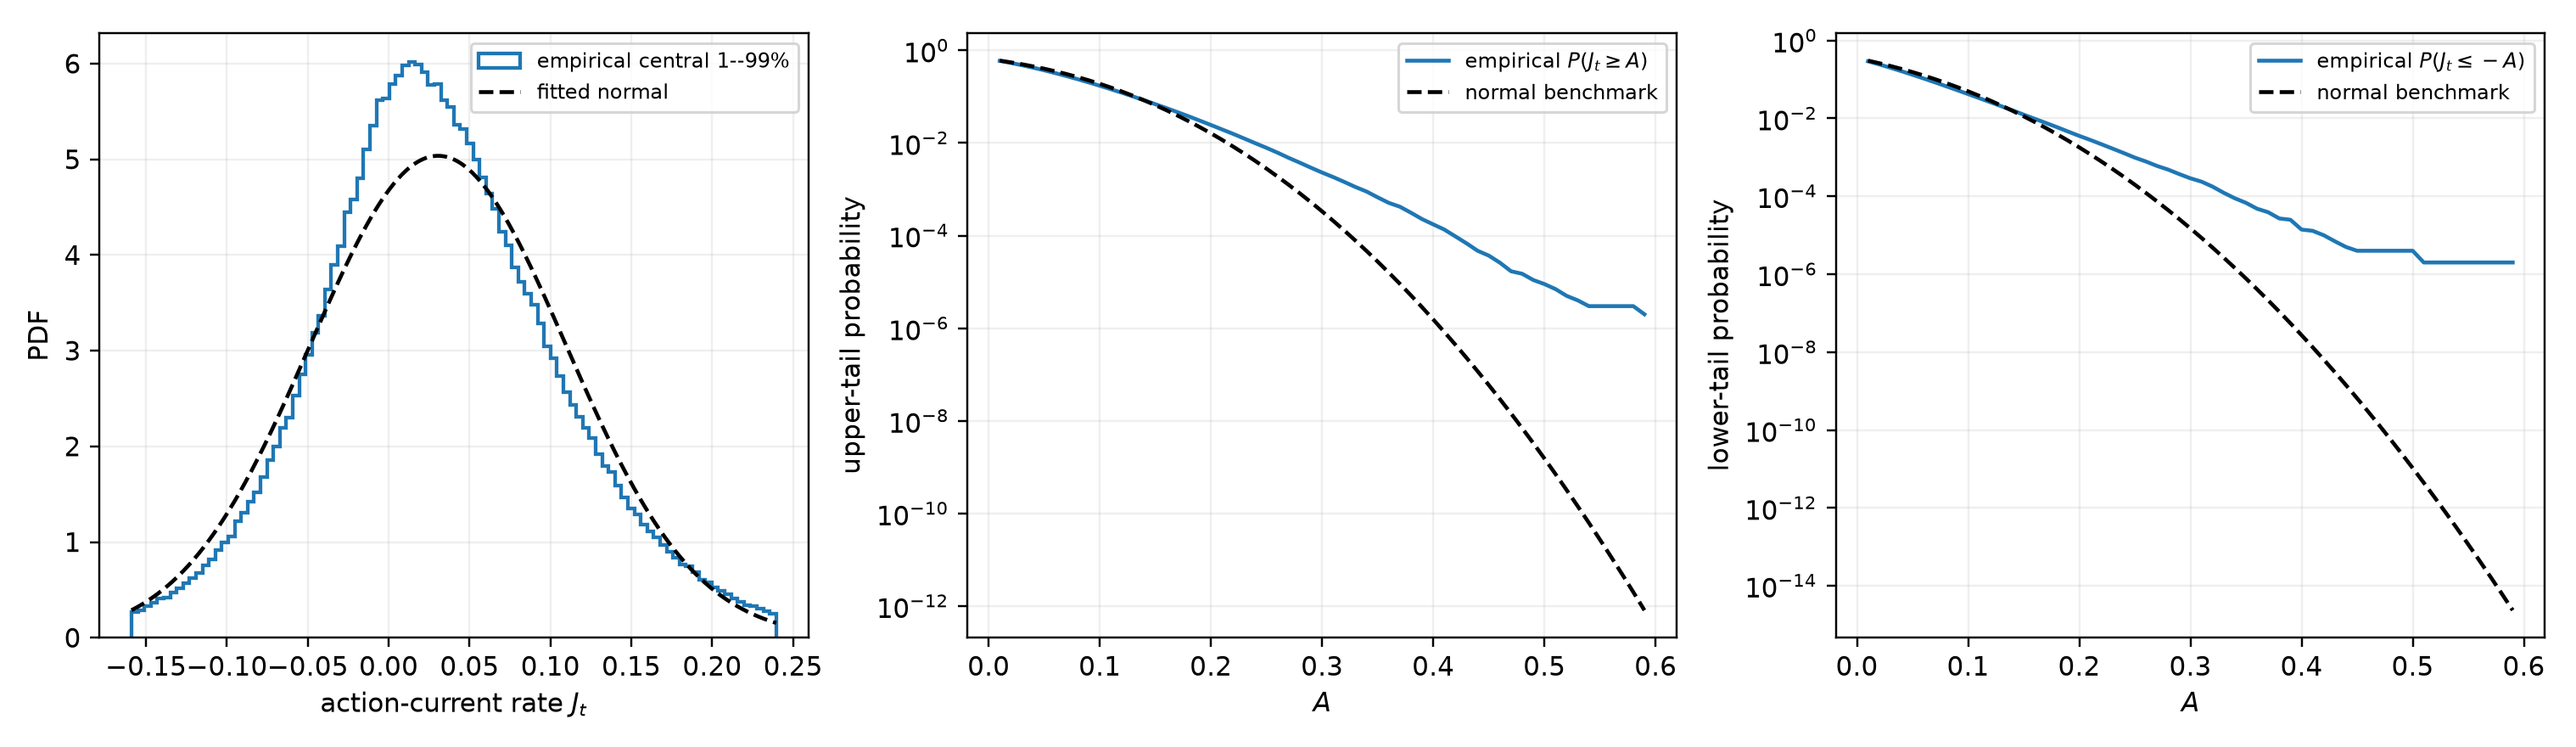
\includegraphics[width=0.48\textwidth]{action_tail_normal_fit_n40_t20.png}
\caption{Representative $\tau=20$ normal-tail comparisons.  Solid empirical
curves and the full-sample Gaussian benchmark disagree in the far tail; the
tail-optimized Gaussian is shown only as a descriptive comparison.}
\label{fig:normal}
\end{figure}

\subsection{Dependence on threshold and averaging time}

For each threshold on the $0.01$ grid, both signs were counted after sorting
the samples.  A fit was allowed only when every included point had at least
20 raw events, probability at most $0.2$, and at least four averaging times.
The fitted form was
\begin{equation}
 \log\Prob(J_\tau\ge A)=b_+(A)-\tau I_+(A),\qquad
 \log\Prob(J_\tau\le-A)=b_-(A)-\tau I_-(A).
 \label{eq:rate-fit}
\end{equation}
Every accepted fit has $R^2\ge0.98$.  The rate proxies $I_\pm(A)$ increase
with threshold magnitude.  The resolved positive-tail ranges are
$[0.46,0.81]$, $[0.15,0.33]$, $[0.08,0.20]$, and $[0.05,0.15]$ for
$n=10,20,30,40$.  Negative-tail fits are resolved over $[0.01,0.06]$ for
$n=20$ and $[0.01,0.08]$ for $n=30,40$.  At $n=10$, the negative current
becomes too rare to sustain four resolved times.

\begin{figure}[ht]
\centering
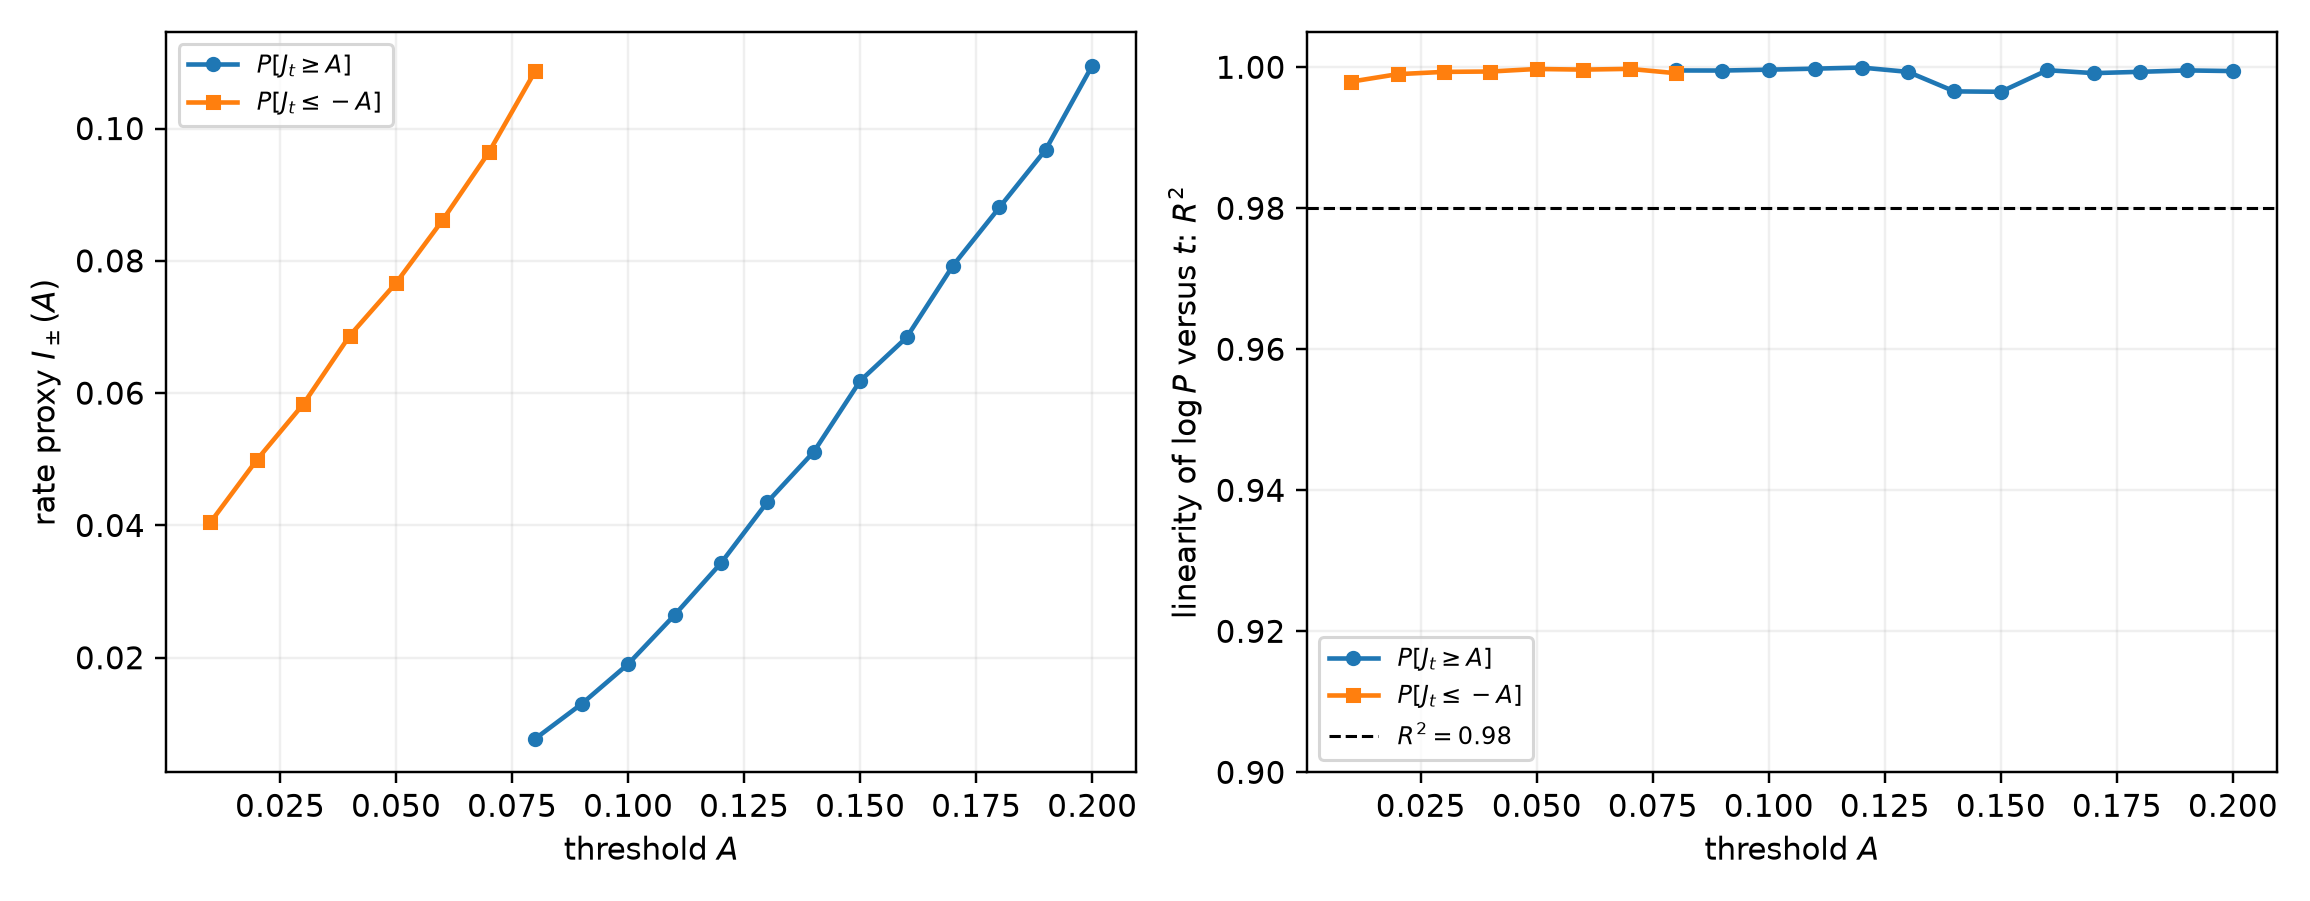
\includegraphics[width=0.72\textwidth]{action_tail_time_scaling_n30.png}
\caption{$n=30$ finite-time rate proxies.  Approximate linearity in $\tau$ at
fixed $A$ is evidence for finite-time large-deviation scaling; it is not by
itself a fluctuation theorem.}
\label{fig:time-scaling}
\end{figure}

The answer to ``how does $\log P$ depend on $A$ and $\tau$?'' is therefore:
at fixed $A$, the resolved rare-tail log probability is approximately linear
in $\tau$; at fixed $\tau$, it is curved in $A$, so one exponential in $A$
does not describe the whole tail.  In large-deviation notation,
\begin{equation}
 \Prob(J_\tau\approx A)\asymp e^{-\tau I(A)},
\end{equation}
with a nonlinear rate function $I(A)$.

\subsection{Direct fluctuation-symmetry result}

For the medium-entropy rate $a=\sm_\tau/\tau$, the simple asymptotic reference
is
\begin{equation}
 \frac1\tau\log\frac{p_\tau(a)}{p_\tau(-a)}=a.
 \label{eq:direct-ft}
\end{equation}
The directly fitted slopes are below one.  At $\tau=20$, they are
$0.653,0.341,0.247,$ and $0.208$ for $n=10,20,30,40$.  Where the negative
tail remains well resolved they initially move upward with $\tau$; for
example, the $n=30$ slopes are $0.247,0.316,$ and $0.393$ at
$\tau=20,40,60$.  They do not reach one before the two-sided histogram loses
support.

\begin{table}[ht]
\centering
\scriptsize
\begin{tabular}{rrrrrr}
\toprule
$n$ & $N_-(\sm;20)$ & $N_-(\sm;200)$
& $s_{\sm}(20)$ & $s_Q(20)$ & $\Delta\beta$\\
\midrule
10 & 7,158   & 0   & 0.653 & 0.217 & 0.4\\
20 & 107,491 & 0   & 0.341 & 0.126 & 0.4\\
30 & 214,942 & 4   & 0.247 & 0.081 & 0.4\\
40 & 276,375 & 195 & 0.208 & 0.058 & 0.4\\
\bottomrule
\end{tabular}
\caption{Direct-sampling resolution and symmetry diagnostics.  Here
$N_-(X;\tau)$ counts negative blocks, while $s_{\sm}$ and $s_Q$ are the
fitted antisymmetry slopes.  Sparse later tails are not replaced by normal
extrapolation or plus-four counts.}
\label{tab:direct-ft}
\end{table}

\begin{figure}[ht]
\centering
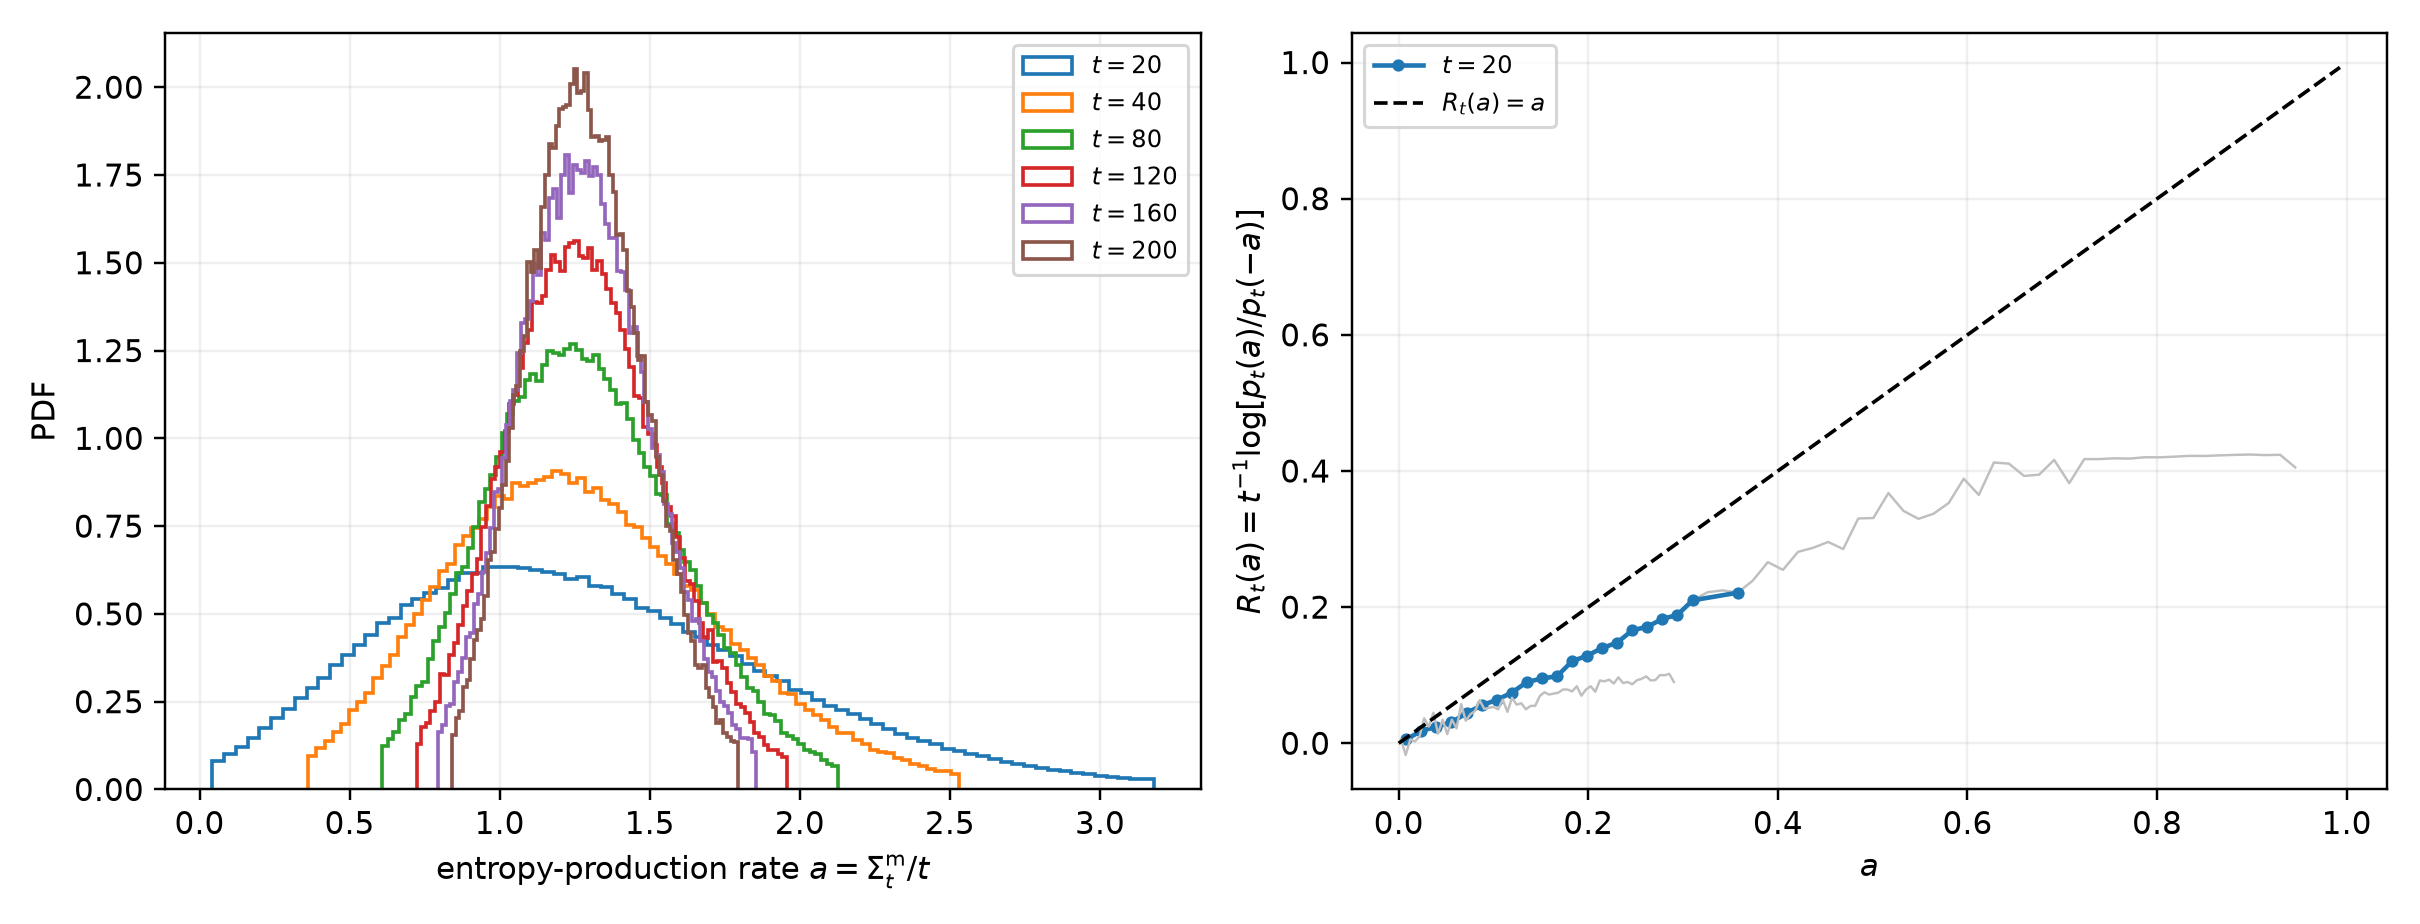
\includegraphics[width=0.48\textwidth]{entropy_pdf_symmetry_n10.png}\hfill
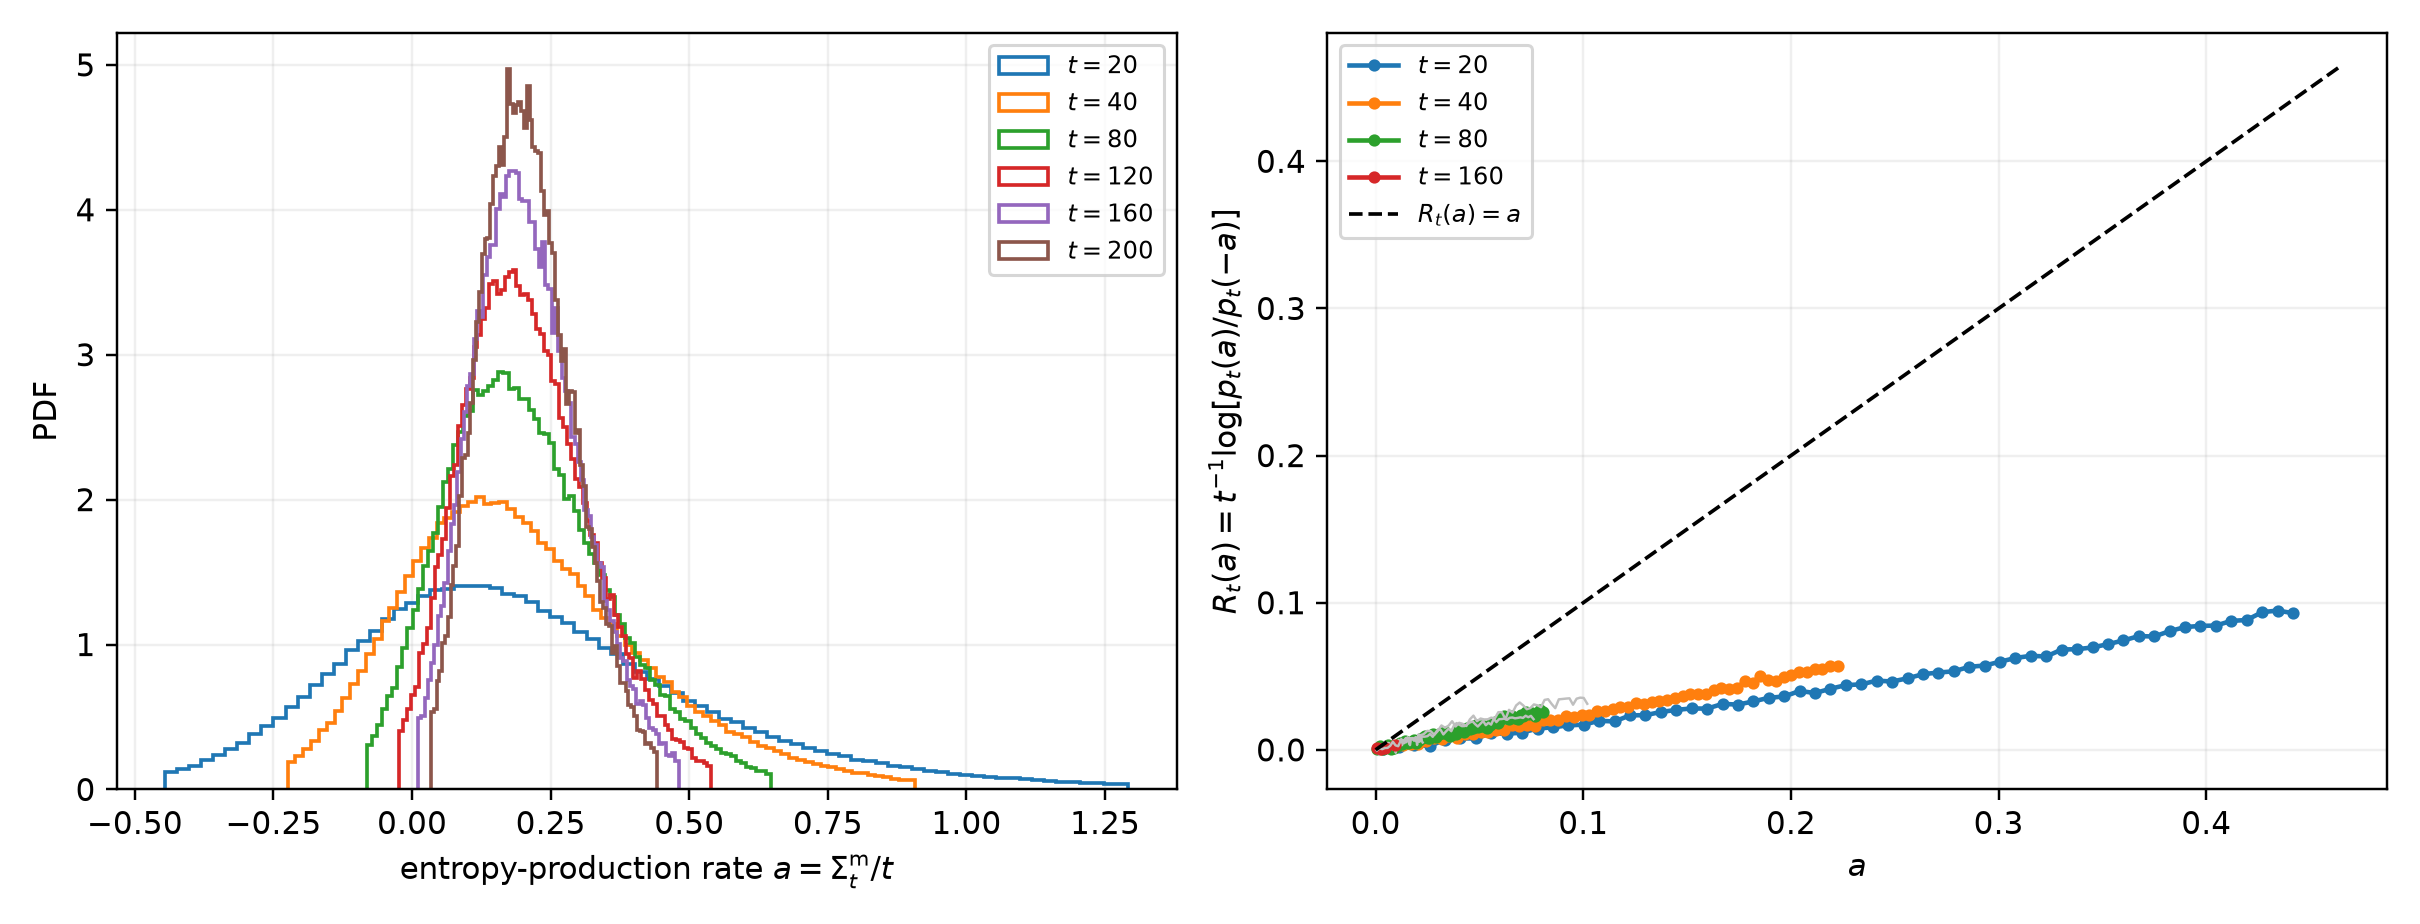
\includegraphics[width=0.48\textwidth]{entropy_pdf_symmetry_n40.png}
\caption{Representative medium-entropy symmetric-bin diagnostics.  The fit
uses only raw nonzero counts from both signs.}
\label{fig:entropy-symmetry}
\end{figure}

This is not evidence that the FT is violated.  An exact finite-time relation
involves the total trajectory entropy
\begin{equation}
 \stot_\tau=\sm_\tau+\log\rho(Z_0)-\log\rho(Z_\tau),
 \label{eq:total}
\end{equation}
whereas the million-block long-chain data do not reconstruct the NESS endpoint
density.  Boundary terms and exponentially vanishing negative-tail support
can therefore prevent medium entropy from displaying the asymptotic symmetry
at accessible times.  The correct direct-sampling conclusion is:
\begin{quote}
The standard thermodynamic symmetry is not verified in the directly sampled
finite-time window.  The observed slope deficit is endpoint- and rare-tail
limited and is not a demonstrated violation.
\end{quote}

\subsection{Action current is not entropy production}

Heat and action become more correlated as the averaging time grows, but they
are not tightly coupled.  At $\tau=200$, the Pearson correlations are
$0.934,0.896,0.803,$ and $0.683$ for $n=10,20,30,40$, while the fraction of
heat variance left after linear regression on action is
$0.128,0.197,0.355,$ and $0.533$.  Consequently, a visually attractive
positive/negative action-current ratio cannot be called a thermodynamic FT,
especially for longer chains.

\section{Finite-time total-entropy controls at \texorpdfstring{$n=2$}{n=2}}

The endpoint issue in \eqref{eq:total} can be addressed at $n=2$, where both
sites are thermostatted and the stationary density can be estimated in a
reduced phase-invariant coordinate system.  The accepted driven calculation
uses $1{,}048{,}576$ non-overlapping blocks of duration $0.1$ after burn-in,
with an independently validated equilibrium data set used to select the
density representation.

The resulting total-entropy detailed-FT fit is
\begin{equation}
 \log\frac{p(s)}{p(-s)}=-0.02219+(0.994496\pm0.00738)s.
\end{equation}
The integral relation gives
\begin{equation}
 \log\E e^{-\stot}=0.002175,
 \qquad 95\%\ \mathrm{CI}=[-0.000744,0.005251],
\end{equation}
with exponential-weight ESS $324{,}604$.  Support, equilibrium-density,
stationarity, sensitivity, and first-law gates pass.

\begin{figure}[ht]
\centering
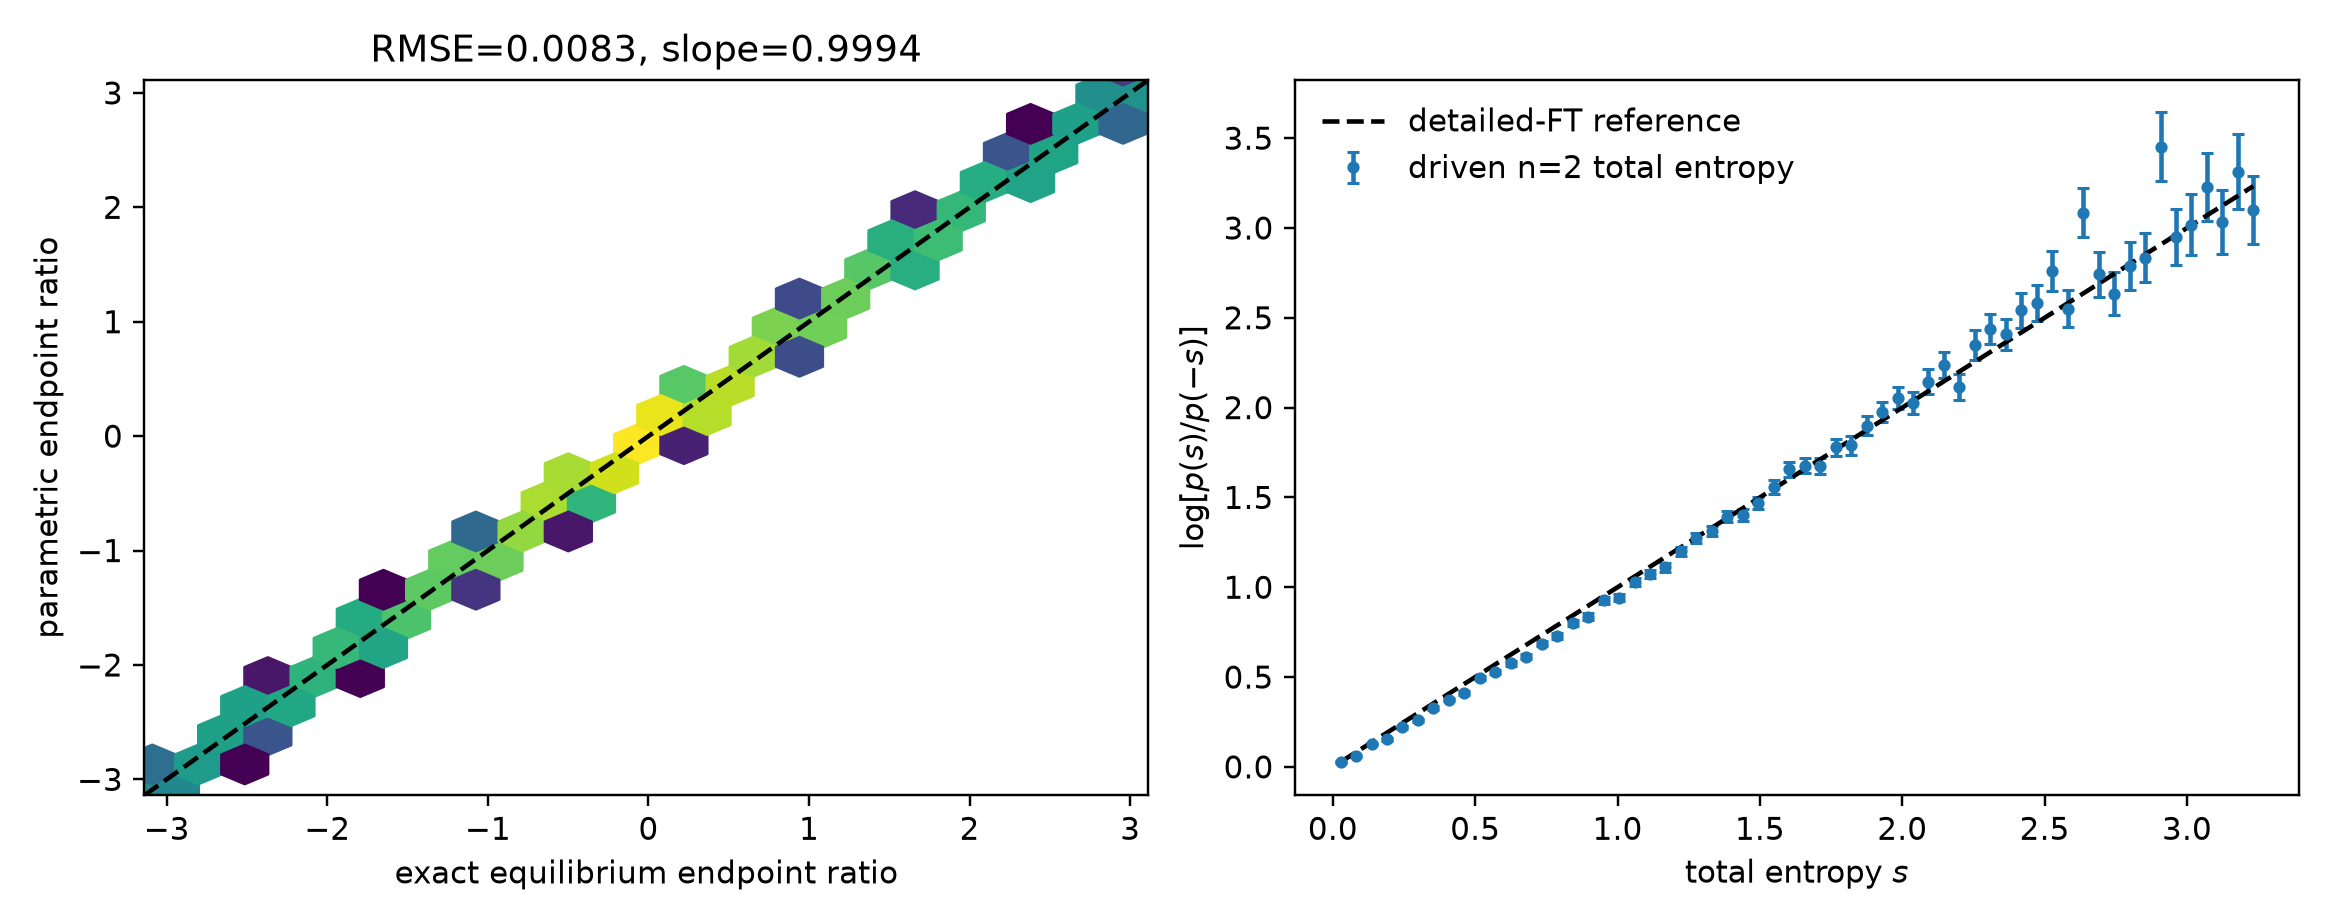
\includegraphics[width=0.78\textwidth]{n2_total_entropy_ft.png}
\caption{Accepted $n=2$ endpoint-density validation and driven NESS
total-entropy detailed relation.}
\label{fig:n2}
\end{figure}

An independent discrete-path calculation avoids stationary-density estimation
entirely.  It accumulates the exact forward/reverse Gaussian transition-kernel
ratio of the split integrator for one million trajectories in each direction.
Its Crooks fit is
\begin{equation}
 \log\frac{p_F(s)}{p_R(-s)}
 =0.000259+(0.993352\pm0.00243)s.
\end{equation}
Both forward and reverse integral relations pass.  Timestep refinement shows
first-order convergence of the exact discrete kernel entropy to the physical
bath-heat entropy.

\begin{figure}[ht]
\centering
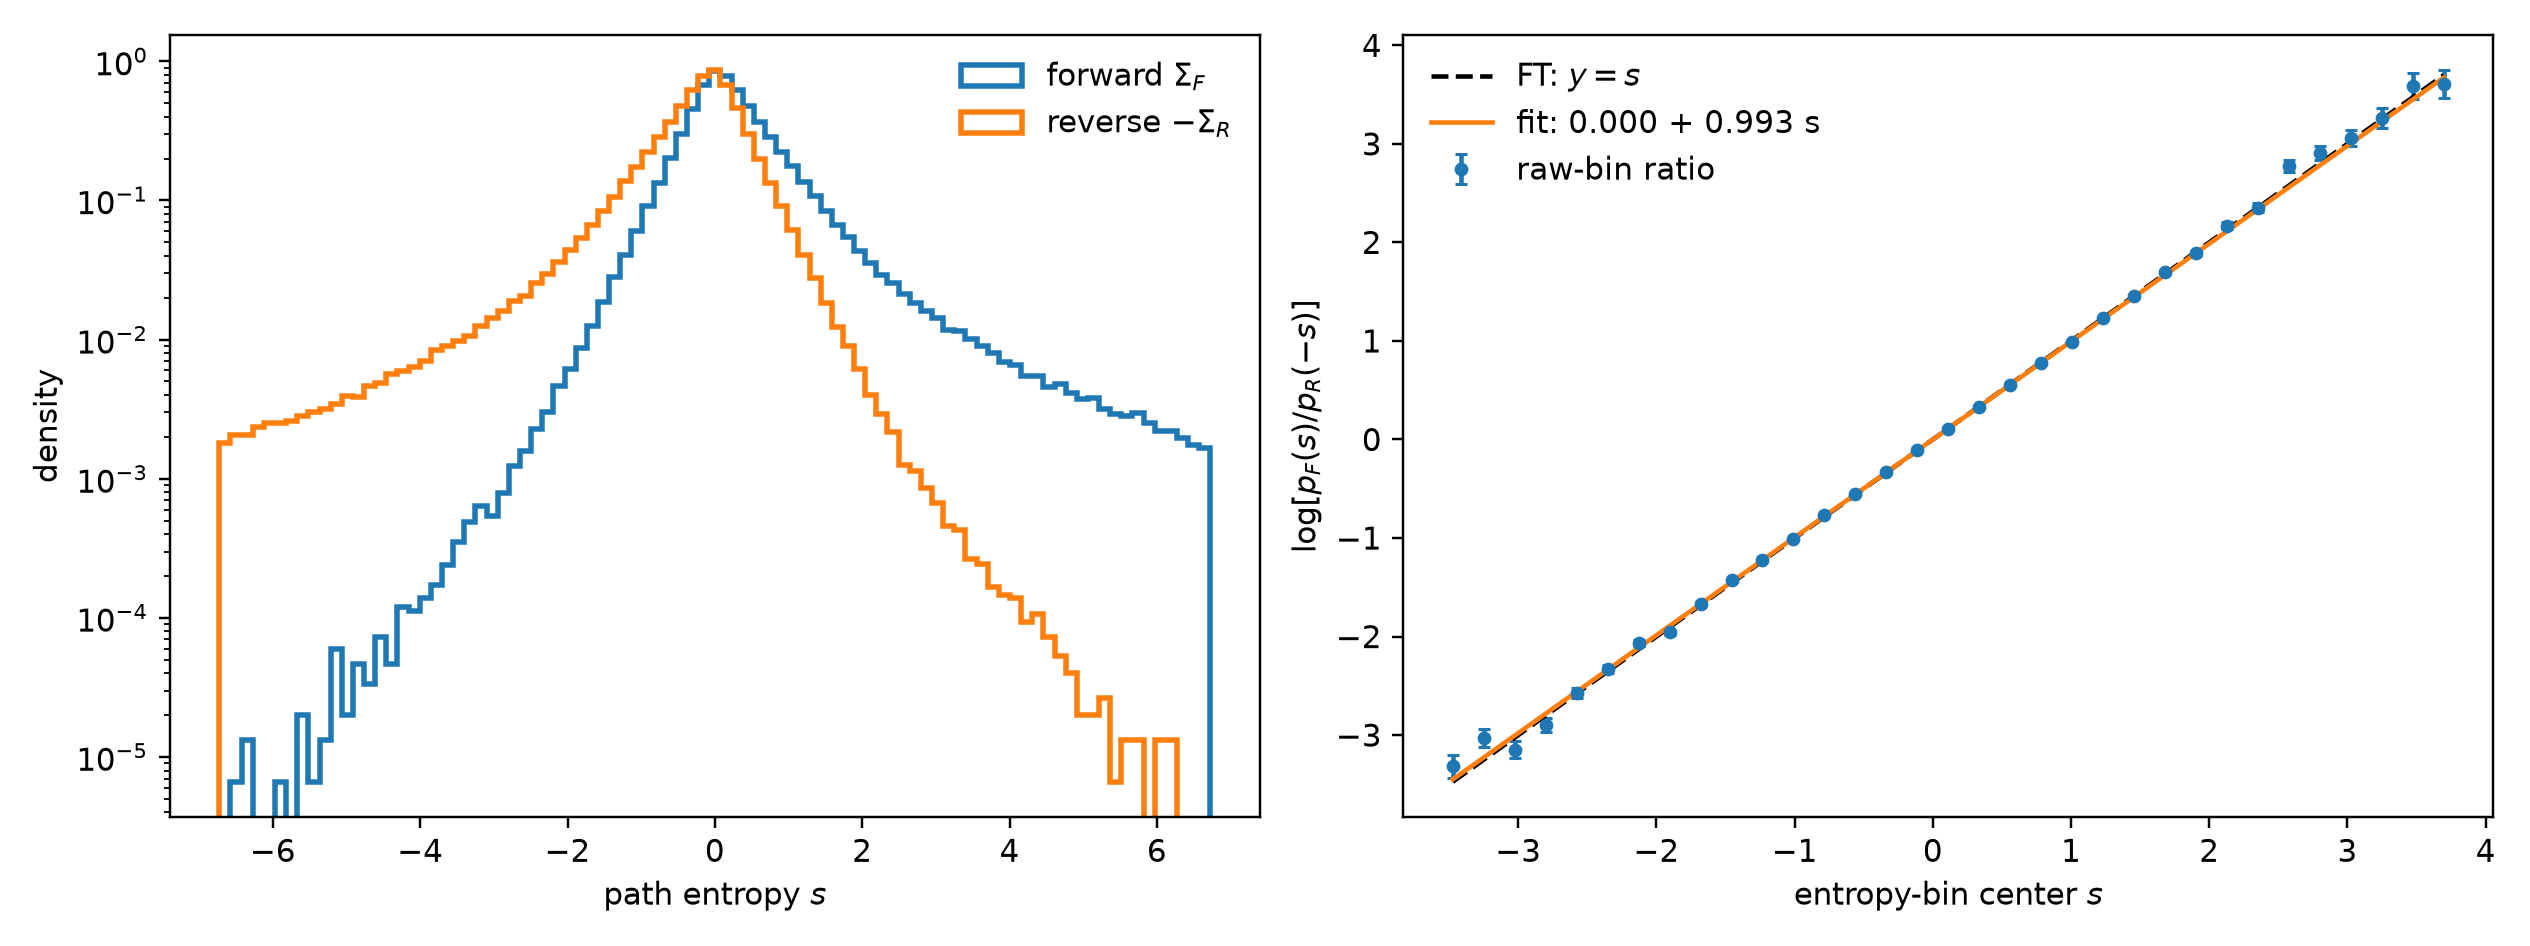
\includegraphics[width=0.63\textwidth]{discrete_path_ft.png}\hfill
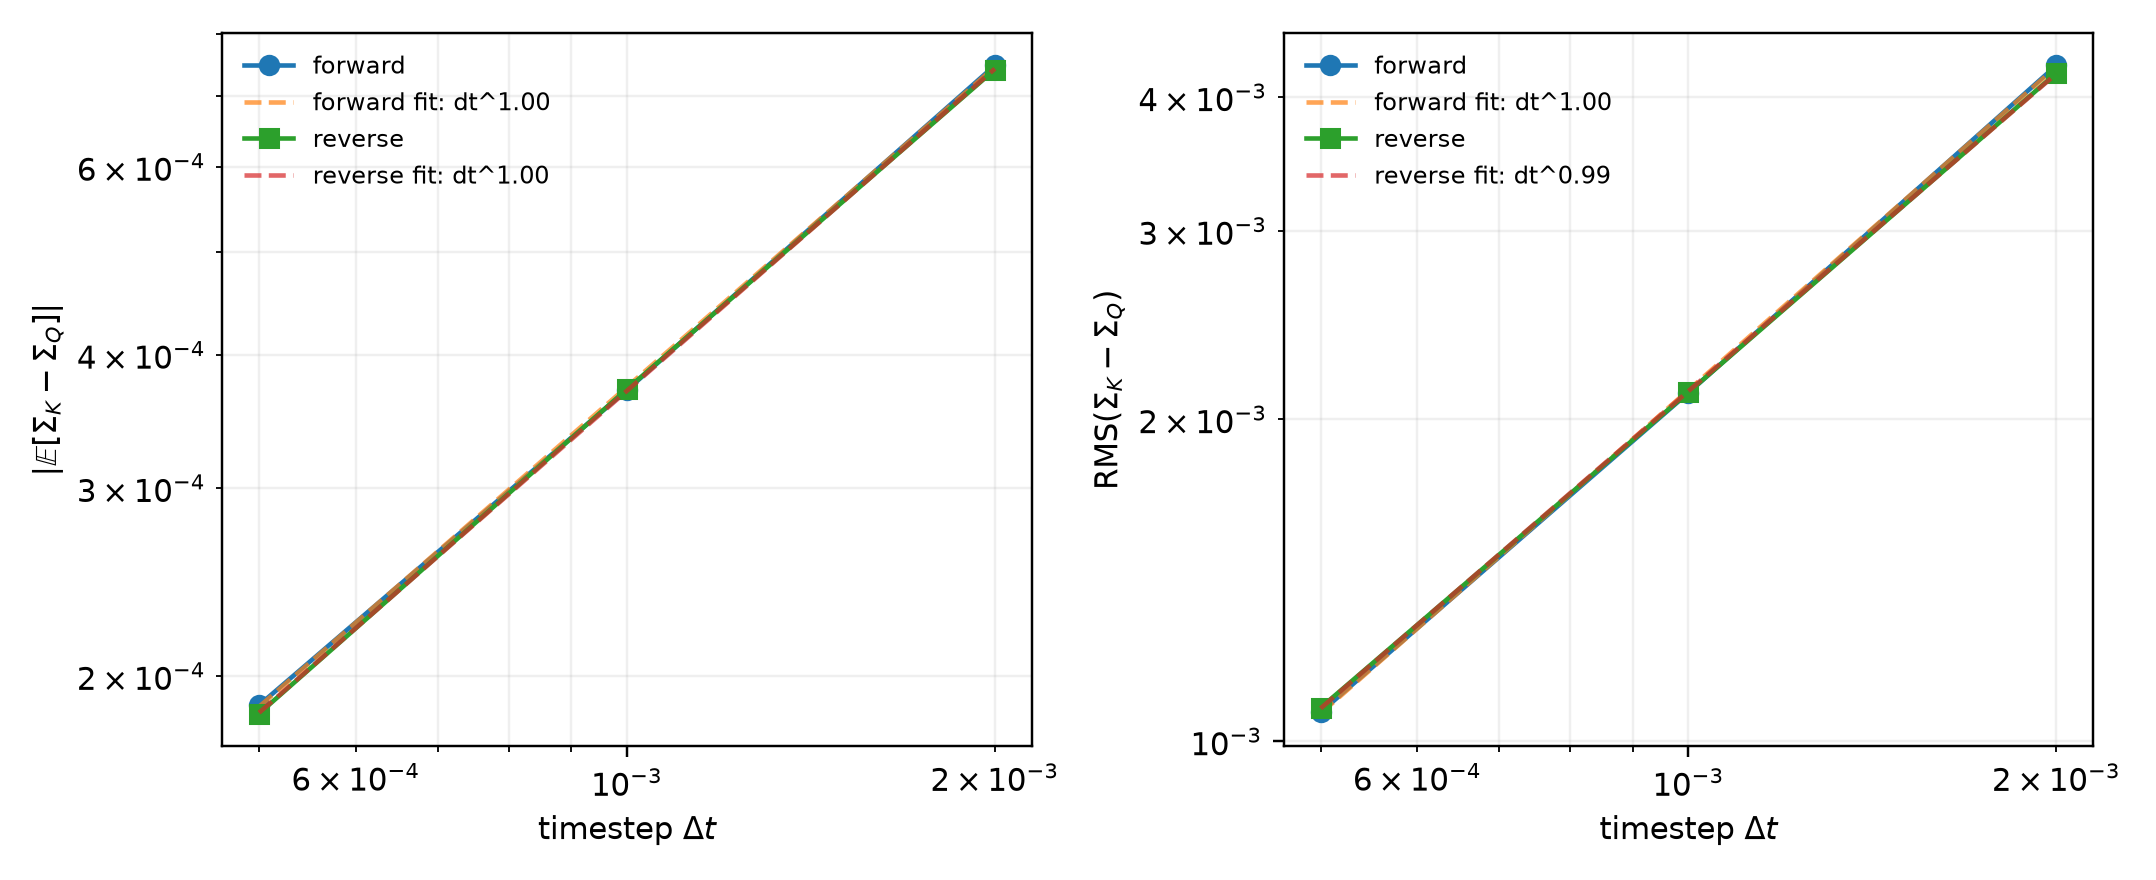
\includegraphics[width=0.34\textwidth]{kernel_heat_timestep_convergence.png}
\caption{Independent finite-step path-ratio FT and its continuous-time heat
interpretation.}
\label{fig:path}
\end{figure}

Together these experiments support a paper-level finite-time numerical claim
for the two-site model.  They do not establish the same statement for a long
chain.

\section{Long-chain Gallavotti--Cohen SCGF test}

Direct sampling cannot efficiently resolve exponentially rare negative tails
at long times.  The long-chain study therefore estimates the scaled cumulant
generating function
\begin{equation}
 \psi_n(k)=\lim_{t\to\infty}\frac1t
 \log\E e^{-k\Sigma_R(t)},
 \qquad \Sigma_R=-(T_R^{-1}-T_L^{-1})Q_R=-0.4Q_R.
\end{equation}
The Gallavotti--Cohen diagnostic is
\begin{equation}
 \psi_n(k)=\psi_n(1-k).
 \label{eq:gc}
\end{equation}

The cloning protocol freezes complementary tilts, four independent seeds per
member, support thresholds, observation horizons, and population, timestep,
and selection-interval controls.  Phase II contains 56 complete summaries,
56 timeseries, and 56 logs.  No output is malformed or nonfinite, no midpoint
solve fails, and all prospective gates pass.

\begin{table}[ht]
\centering
\small
\begin{tabular}{rrrrrrc}
\toprule
$n$ & $(k,1-k)$ & clones & horizon & $\psi(k)-\psi(1-k)$ & 95\% CI & gates\\
\midrule
10 & $(0.3,0.7)$ & 2048 & 60  & $-0.000075$ & $[-0.009953,\ 0.009802]$ & pass\\
20 & $(0.4,0.6)$ & 1024 & 60  & $-0.003389$ & $[-0.012081,\ 0.005302]$ & pass\\
30 & $(0.4,0.6)$ & 4096 & 60  & $-0.002336$ & $[-0.007251,\ 0.002578]$ & pass\\
40 & $(0.4,0.6)$ & 1024 & 120 & $+0.004498$ & $[-0.002343,\ 0.011340]$ & pass\\
\bottomrule
\end{tabular}
\caption{Final long-chain paired SCGF residuals.  ``Pass'' includes support,
time, population, timestep, and selection controls applicable to that row.}
\label{tab:gc}
\end{table}

\begin{figure}[ht]
\centering
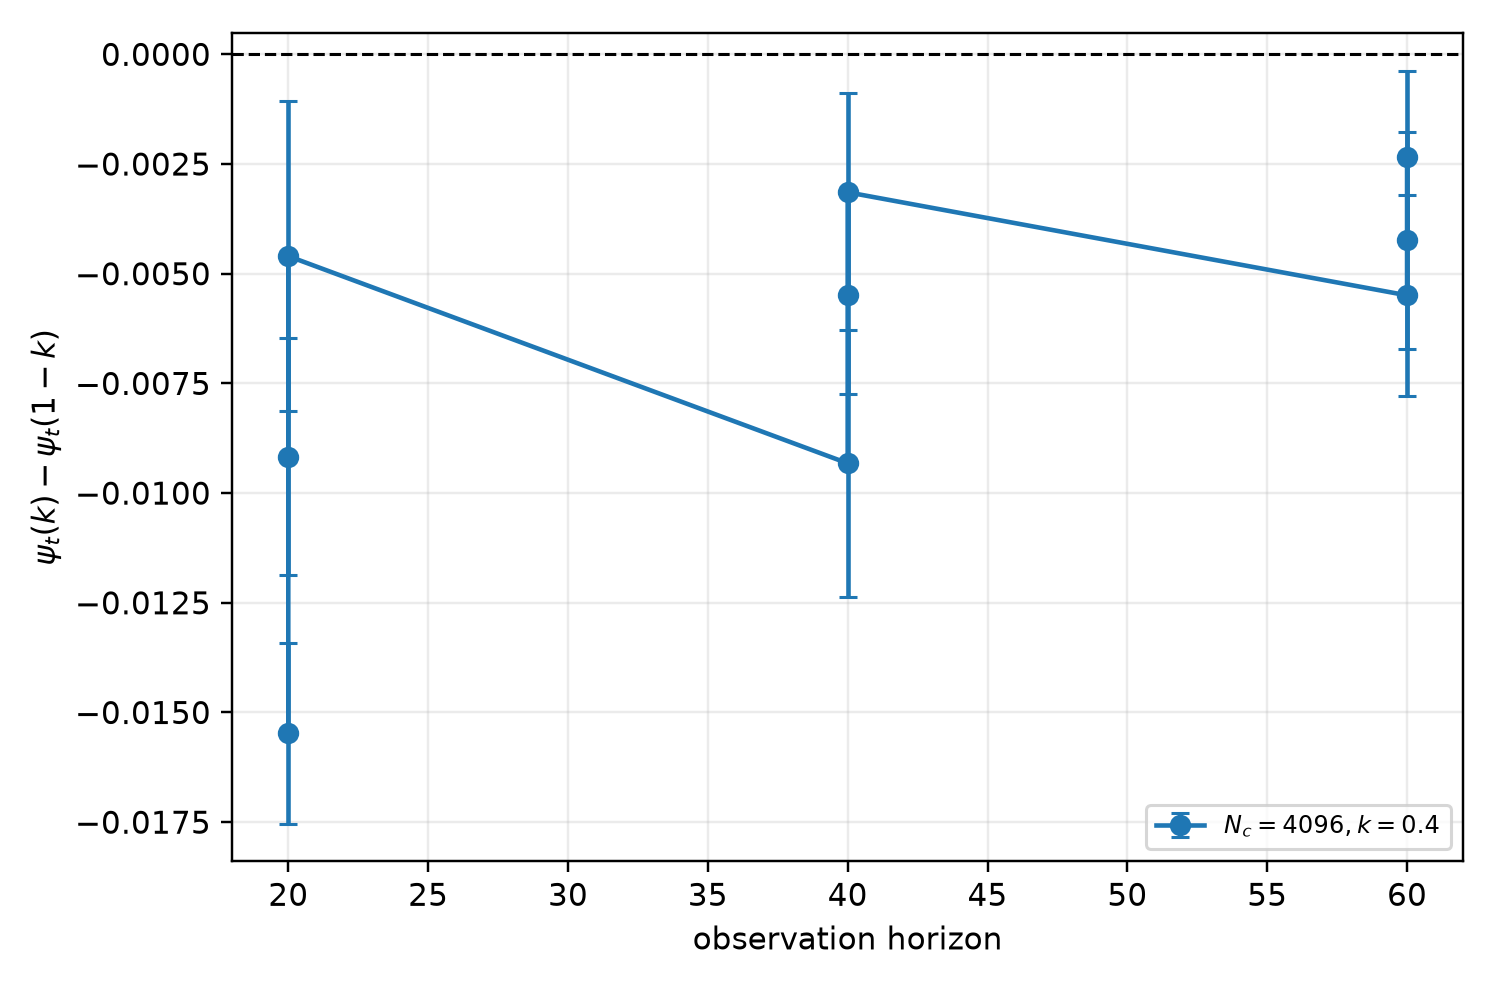
\includegraphics[width=0.78\textwidth]{n30_gc_convergence.png}
\caption{$n=30$ observation-time, population, timestep, and selection
convergence of the paired SCGF residual.}
\label{fig:n30}
\end{figure}

Every confidence interval in Table~\ref{tab:gc} contains zero and every
absolute residual is below the frozen tolerance.  The normalized residuals
are approximately $-0.04\%,-4.0\%,-4.9\%,$ and $12.9\%$.  The $n=40$
absolute gate passes, but its relative uncertainty is larger because the SCGF
magnitude is smaller.  This caveat must remain visible.

The admissible long-chain claim is:
\begin{quote}
For the boundary-driven projection-free Cartesian NLS chain at
$(T_L,T_R,\gamma)=(10,2,0.1)$, controlled rare-event estimates are consistent
with Gallavotti--Cohen SCGF symmetry at all four tested finite chain lengths
over the resolved complementary tilt pair.
\end{quote}

It is not legitimate to claim exact equality, symmetry over all
$k\in[0,1]$, uniformity in $n$, or an $n\to\infty$ theorem from these data.

\section{Final answer to the second-round questions}

\begin{enumerate}
\item \textbf{Was the requested sampling completed?} Yes.  The requested
million-sample scale was reached for all four chain lengths, with complete
heat, entropy, current, endpoint-audit, and stream metadata.
\item \textbf{What is the flux distribution?} Its centre becomes
Gaussian-like under longer averaging, while the $\tau=20$ far tails are
heavier than the full-sample Gaussian benchmark.
\item \textbf{How does $\log P$ depend on $A$ and $\tau$?} At fixed resolved
$A$, it is approximately affine in $\tau$; the fitted decay rate grows with
$|A|$.  At fixed $\tau$, the dependence on $A$ is curved, consistent with a
nonlinear finite-time rate function.
\item \textbf{Does the directly sampled current obey the FT?} The direct
medium-entropy and heat ratios do not reach their references in the accessible
window.  This is an unresolved finite-time test, not a demonstrated failure.
Action-current symmetry has no thermodynamic target.
\item \textbf{Can the FT be verified numerically at all?} Yes, with scoped
observables.  At $n=2$, total entropy passes two independent finite-time
checks.  At $n=10,20,30,40$, long-time entropy-current cloning is consistent
with the GC SCGF symmetry at the tested pairs after all frozen controls.
\end{enumerate}

\section{Code, data, and provenance map}

\begin{table}[ht]
\centering
\scriptsize
\begin{tabularx}{\textwidth}{>{\raggedright\arraybackslash}p{0.19\textwidth}
>{\raggedright\arraybackslash}p{0.37\textwidth}X}
\toprule
Module & Principal code & Accepted results\\
\midrule
Direct tails & \path{code/direct_sampling/NLS_entropy_ft.cpp},
\path{analyze_entropy_ft.py}, \path{plot_entropy_ft_supplement.py},
\path{analyze_action_tail_time_scaling.py} &
\path{results/direct_sampling/}\\
$n=2$ endpoint entropy & \path{code/n2_total_entropy/analyze_total_entropy_parametric_n2.py}
and independent audit & \path{results/n2_total_entropy/}\\
Discrete path ratio & \path{code/discrete_path/NLS_discrete_path_ft.cpp} and
\path{analyze_discrete_path_ft.py} & \path{results/discrete_path/}\\
Long-chain SCGF & \path{code/long_chain_scgf/NLS_entropy_cloning.cpp},
\path{analyze_long_chain_ft.py}, \path{analyze_long_chain_ft_controls.py} &
\path{results/long_chain_phase2/}\\
\bottomrule
\end{tabularx}
\caption{Traceability from each scientific claim to code and accepted data.}
\end{table}

The compact package contains all code, result tables, audits, figures,
protocols, and all Phase-II raw summaries/timeseries.  The multi-gigabyte
block and trajectory CSVs are kept once in the main local repository.  Their
absolute locations, byte counts, and SHA-256 hashes are listed in
\path{RAW_DATA_INDEX.md}.  Reproduction commands are in
\path{REPRODUCE.md}; the package-level integrity list is
\path{SHA256SUMS.txt}.

\section*{Claim boundary for manuscript use}

The direct distribution study can be reported as finite-time current
fluctuations and large-deviation evidence.  The $n=2$ result can be reported
as a controlled finite-time total-entropy numerical verification.  The
long-chain result can be reported as controlled numerical consistency with
GC symmetry at the tested complementary pairs.  None of these numerical
results alone proves the continuous-time theorem or the infinite-chain
limit.

\end{document}
